\documentclass[]{article}
\usepackage{amssymb,amsmath}
\usepackage{hyperref}

\usepackage{todonotes}
\usepackage[margin=2.5cm]{geometry}
\usepackage[super]{natbib}
\bibliographystyle{unsrtnat}


\title{Information Theory and Statistical Mechanics}

\author{E. T. Jaynes\\
Washington University}
\date{July 1962}

\begin{document}

BRANDEIS UNIVERSITY SUMMER INSTITUTE\\
LECTURES IN THEORETICAL PHYSICS

K. W. Ford, \emph{\textbf{Editor}}

\begin{enumerate}
\def\labelenumi{\arabic{enumi}.}
\setcounter{enumi}{1959}
\item
  Lectures

\begin{quote}
C. Miller • P. T. Matthews • J. Schwinger • N. Fukuda • J. J. Sakurai
\end{quote}

\item Lectures
  \begin{quote}
  \emph{\textbf{Vol. 1}}
R. J. Eden • J. C. Polkinghorne • G. Källén • J. J.Sakurai
\end{quote}


\begin{quote}
\emph{\textbf{Vol. 2}}
M. E. Rose • E. C. G. Sudarshan
\end{quote}

\item
  Lectures

\begin{quote}
\emph{\textbf{Vol. 1---Elementary Particle Physics and Field Theory}} T.
Fulton • G. Kallen • J. D. Jackson • C. Fronsdal

\emph{\textbf{Vol. 2---Astrophysics and ihe Many-Uody Problem}} E. N.
Parker • J. S. Goldstein • A. A. Maiadudin • V. Anibcgaokar

\emph{\textbf{Vol. 3---Statistical Physics}} G. E. Uhlenbeck • N.
Rosenzwcig • A. J. F Siegert • E. T. Jaynes • S. Fujita
\end{quote}

\end{enumerate}
\pagebreak

Brandeis Summer Institute 1962

STATISTICAL

PHYSICS

3

G. E. Uhlenbeck N. Hosenzweig A. J, F. Siegert E. T. Jaynes S. Fujita

\emph{\textbf{W. A.}} BENJAMIN, INC\emph{\textbf{.}} 
\pagebreak

\twocolumn

STATISTICAL PHYSICS

\begin{quote}
1962 Brandeis Lectures in Theoretical Physics, Volume 3

G. E. Uhlenbeck, N. Rosenzweig, A. J. F. Siegert, E. T. Jaynes, and C.
Fujita.
\end{quote}

In his course on SELECTED TOPICS IN STATISTICAL MECHANICS, Professor G.
E. Uhlenbeck begins with an exposition of some diagrammatic methods used
to calculate virial coefficients and the equation of state. He then
gives a detailed analysis of the mathematics of phase transition with a
soluble one-dimensional model.

The second set of lectures, by Dr. N. Rosenzweig, STATISTICAL MECHANICS
OF EQUALLY LIKELY QUANTUM SYSTEMS, is a discussion of the statistical
properties of energy levels and eigenfunctions for heavy nuclei and
complex atoms, stressing the role of time reversal and other symmetries.

Professor A. J. F. Siegert lectures on FUNCTIONAL INTEGRALS IN
STATISTICAL MECHANICS, demonstrating the utility of new techniques by
analysis of the partition function of the Ising model with long range
interactions.

Information theory has provided the long hoped for algorithm analogous
to the partition sum of equilibrium theory, for calculation of
irreversible processes. The lectures of Professor E. T. Jaynes,
INFORMATION THEORY AND STATISTICAL MECHANICS, provide an introduction to
this subject.

In the final set of lectures, Professor C. Fujita reviews and compares
the independent achievements of Van Hove and Prigogine and their
schools, in their progress toward better understanding the APPROACH TO
EQUILIBRIUM OF A MANY-PARTICLE SYSTEM.


\pagebreak
\onecolumn

\section*{Foreword}

It is now an established tradition of the Brandeis Summer Institute in
Theoretical Physics to have lecturers who present a systematic account
of recent research in various fields of theoretical physics. The lecture
notes have also become a part of tins tradition, and, although these are
sometimes but a first approximation to the spoken lecture, they may
serve to bring these much needed expositions to the wider audience of
physicists who may aspire to contribute to these fields.

I should like to take this opportunity to thank all those whose
participation in the Institute during the summer of 1962 helped maintain
these traditions. Particular words of appreciation are due the National
Science Foundation, for its indispensable financial support, and
Professor Kenneth Ford, who graciously carried the responsibility for
getting the notes ready for publication.

In this volume, the notes of Professor Jaynes and Professor Fujita have
been prepared by the lecturers; Professor Uhlenbeck, Dr. Rosenzweig, and
Professor Siegert have kindly checked over the notes based on their
lectures.

\begin{quote}
\emph{\textbf{\textsc{David L. Falkoff}}} Co-Director of the
\emph{\textbf{1962}} Institute
\end{quote}

\maketitle 

Notes by the lecturer
\pagebreak

\tableofcontents

\section{Introduction}\label{introduction}

At the beginning of every problem in probability theory, there arises a
need to assign some initial probability distribution; or what is the
same thing, to ``set up an ensemble.'' This is a problem which cannot be
evaded, and for which the laws of physics give us no help. For example,
the laws of physics tell us that a density matrix
\(\rho\left( t \right)\) must vary with time according to
\(\dot{\rho} = \lbrack H,\rho\rbrack\), but they do not
tell us what function \(\rho(0)\) should be put in at the start.
Assignment of \(\rho(0)\) is, of course, a matter of free choice on our
part---it is for us to say which problem we want to solve.

The assignment of initial probabilities must, in order to be useful,
agree with the initial information we have (i.e., the results of
measurements of certain parameters). For example, we might know that at
time \(t = 0\), a nuclear spin system having total (measured) magnetic
moment \(M(0)\), is placed in a magnetic field \(H\), and the problem is
to predict the subsequent variation \(M(t)\), which presumably tends to
an equilibrium value \(M\left( \infty \right) = x_{0}H\) after a long
time. What initial density matrix for the spin system \(\rho(0)\),
should we use? Evidently, we shall want it to satisfy, at the very
least,

\begin{equation}
\text{Tr}\left( \rho(0)M_{o_{p}} \right) = M(0) \label{eqn-one}
\end{equation}

where \(M_{o_p}\) is the operator corresponding to total magnetic moment. But Eq. (\ref{eqn-one}) is very far from uniquely
specifying \(\rho(0)\). Out of the infinite number of density matrices
satisfying (\ref{eqn-one}), which should we choose as the starting point of our
calculation to predict \(M(t)\)?

Conventional quantum theory has provided an answer to the problem of
setting up initial state descriptions only in the limiting case where
measurements of a ``complete set of commuting observables'' have been
made, the density matrix \(\rho(0)\) then reducing to the projection
operator onto a pure state \(\psi(0)\) which is the appropriate
simultaneous eigenstate of all the measured quantities. But there is
almost no experimental situation in which we really have all this
information, and before we have a theory able to treat actual
experimental situations, existing quantum theory must be supplemented
with some principle that tells us how to translate, or encode, the
results of measurements into a definite state description \(\rho(0)\).
Note that the problem is not to find the \(\rho(0)\) which correctly
describes the "true physical situation." That is unknown, and always
remains so, because of incomplete information. In order to have a usable
theory we must ask the much more modest question: ``What \(\rho(0)\) best
describes our \emph{state of knowledge} about the physical situation?''

In order to emphasize that this problem really has nothing to do with
the laws of physics (and, as a corollary, that its solution will have
applications outside the field of physics), consider the following
problem. A die has been tossed a very large number \(N\) of times, and
we are told that the \emph{average} number of spots up per toss was not
3.5, as we might expect from an honest die, but 4.5. Translate this
information into a probability assignment
\(P_{n},n = 1,\ 2,\ \ldots,6\), for the \(n\)th face to come up on the
next toss.

To explain more fully what is meant by this, note that we are \emph{not} asking
for an estimate of the fraction (i.e., the relative frequency) of tosses
which give \(n\) spots There is, indeed, a connection between the
probability and the frequency, which we will derive later. But the
problem stated is to reason as best we can about the \emph{individual}
case. The probability \(P_{n}\) must therefore be interpreted in the
so-called "subjective" sense; it is only a means of describing how
strongly we \emph{believe} that the \(n\)-th face will come up in the
next toss.

To state the problem more drastically, imagine that we are offered
several bets, at various odds, on various values of \(n\), and we are
compelled to accept one of these bets. The probabilities \(P_{n}\) are
the basic raw material from which we decide which one to accept. This is
typical of many practical problems faced by the scientist, the engineer,
the statistician, the politician; and indeed all of us. We are
continually faced with situations where some definite decision must be
made \emph{now}, even though we do not have all the information we might
like.

%
\begin{figure}
    \centering
    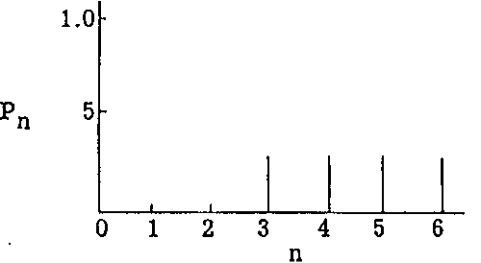
\includegraphics[width=3.20866in,height=1.75197in]{media/image1.jpeg}
    \caption{}
    \label{fig-one}
\end{figure}
%
\begin{figure}
    \centering
    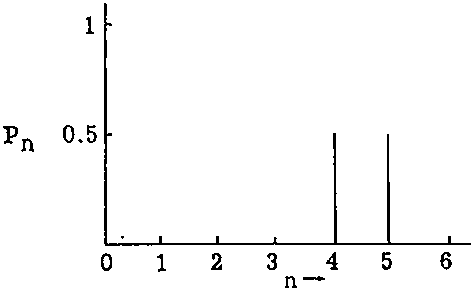
\includegraphics[width=3.16142in,height=2in]{media/image2.png}
    \caption{}
    \label{fig-two}
\end{figure}

Conventional probability theory does not provide any principle for assigning the probabilities $P_n$; so let us think about it a little. We must evidently, choose $P_n$ such that
\begin{align}
\sum_{n = 1}^{6} P_{n} = & 1  \label{eqn-two} \\
\sum_{n = 1}^{6} nP_{n} = & 4.5 \label{eqn-three}
\end{align}
where (\ref{eqn-three}) is analogous to (\ref{eqn-one}). A possible solution of (\ref{eqn-two}) and (\ref{eqn-three}) is indicated
in Fig. \ref{fig-one}; we could take \(P_{4} = P_{5} = 1/2\), all other
\(P_{n} = 0\), This agrees with all the given data. But our common sense
tells us it is not a \emph{reasonable} assignment. The assignment of
Fig. \ref{fig-two} is evidently a more honest description of what we know. But even
this is not reasonable---nothing in the data tells us that n = 1, 2 are
impossible events. In Fig. \ref{fig-two}, we are still jumping to conclusions not
warranted by the available evidence. Evidently, it is unreasonable to
assign probability zero to \emph{any} situation unless our data really rules
out that case. If we assign \(P_{1} > 0\), \(P_{2} > 0\), then in order
to keep the average at 4.5, we shall have to give some increased weight
to the cases \(n = 5,\ 6\). Figure \ref{fig-three} shows an assignment that agrees
with the data and does not ignore any possibility. But it still seems
unreasonable to give the case \(n = 6\) such exceptional treatment.
Figure \ref{fig-four} represents what we should probably call a
backward step---nothing in the data of the problem indicates any reason for such
an uneven treatment. A reasonable assignment \(P_{n}\) must not only
agree with the data and must not ignore any possibility---but
it must also not give undue emphasis to any possibility. The \(P_{n}\)
should vary as smoothly as possible, in some sense. One criterion of
"smoothness" might be that adjacent differences \(P_{n + 1} - P_{n}\)
should be constant; and, indeed, there is a solution with that property.
It is given by \(P_{n} = (12n - 7)/210\) and
is
shown in Fig. \ref{fig-five}. This is evidently the most reasonable probability
assignment so far. But there is a limit to how high an average you can
get with this linear variation of \(P_{n}\). If we took the extreme
case, \(P_{n} = (\text{const.})(n - 1)\), we should again violate one of our
principles because \(P_{1} = 0\), and the average would be only
\(\sum_{n}^{}{P_{n} = 70/15} = 4.67\). Suppose the data of the problem
had been changed so that the average is to be 4.7 instead of 4.5. Then
there is \emph{no} straight-line solution satisfying \(P_{n} \geq 0\). The
\(P_{n}\) must lie on some concave curve, as in Fig. 6. But the
principles by which we reason
surely are the same whether the data specify 4.5 or 4.7; so it appears that a
result qualitatively such as Fig. \ref{fig-six} should be used also when
\(n = 4.5\).

\begin{figure}
    \centering
    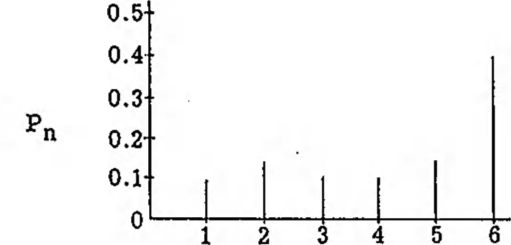
\includegraphics[width=3.39764in,height=1.64567in]{media/image3.jpeg}
    \caption{}
    \label{fig-three}
\end{figure}
\begin{figure}
    \centering
    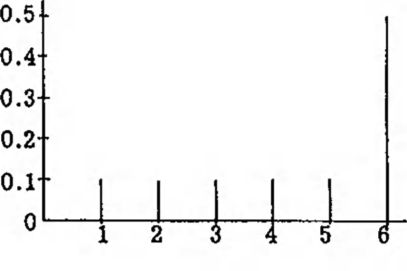
\includegraphics[width=2.71319in,height=1.81042in]{media/image4.jpeg}
    \caption{}
    \label{fig-four}
\end{figure}
\begin{figure}
    \centering
    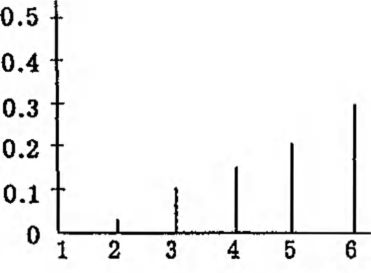
\includegraphics[width=2.48031in,height=1.82283in]{media/image5.jpeg}
    \caption{}
    \label{fig-five}
\end{figure}
\begin{figure}
    \centering
    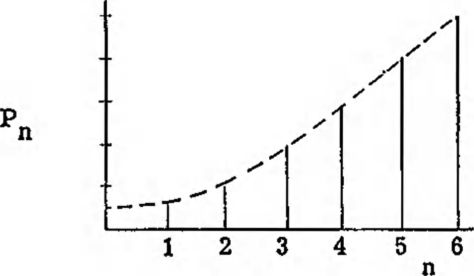
\includegraphics[width=3.16535in,height=1.84252in]{media/image6.jpeg}
    \caption{}
    \label{fig-six}
\end{figure}


This is about as far as qualitative reasoning can take us, and I have carried the argument through on that basis in order to show how ordinary common sense leads us to a result that has all the important features of the quantitative solution given below. The probability assignment $P _{ n }$ which most honestly describes what we know is the one that is as smooth and "spread out" as possible subject to the data. It is the most conservative assignment in the sense that it does not permit one to draw any conclusions not warranted by the data.

This suggests that the problem is a variational one; we need a measure of the "spread" of a probability distribution which we can maximize, subject to constraints which represent the available information. It is by now amply demonstrated by many workers that the "information measure" introduced by Shannon\citep{Shannon-mathematical48} has special properties of consistency and uniqueness which make it \emph{the} correct measure of "amount of uncertainty" in a probability distribution. This is, of course, the expression
%
\begin{equation}
S_{I} = - \sum_{i}^{} p_{i}\log p_{i}
\end{equation}
%
which, \emph{for some distributions} and \emph{in some physical situations}, has long been recognized as representing entropy. However, we have to emphasize that "information-theory entropy" $S _{ I }$ and the experimental thermodynamic entropy $S _{e}$ are entirely different concepts. Our job cannot be to \emph{postulate} any relation between them; it is rather to \emph{deduce} whatever relations we can from known mathematical and physical facts. Confusion about the relation between entropy and probability has been one of the main stumbling blocks in developing a general theory of irreversibility.

\section{The General Maximum-Entropy Formalism}\label{the-general-maximum-entropy-formalism}

To generalize the above problem somewhat, suppose that the quantity
\(x\) can take on the values \((x_1, x_2, \dots x_n)\) where $n$ can be finite or
infinite, and that the average values of several functions $(f_1(x), f_2(x), \dots f_m(x)$ are given, where $m < n$. The problem is to find the probability assignment $p_i =
p(x_i)$ which satisfies the given data: $p_i \geq 0$,
%
\begin{equation}
\sum_{i = 1}^{n} p_{i} = 1 \label{eqn-five}
\end{equation}
\begin{equation}
\sum_{i = 1}^{n}  p_{i}f_{k}\left( x_{i} \right) = \left\langle f_{k}(x) \right\rangle = F_{k} \quad k = 1,2,\ldots,m \label{eqn-six}
\end{equation}
%
and, subject to (\ref{eqn-five}) and (\ref{eqn-six}), maximizes the entropy
%
\begin{equation}
S_{I} = - \sum_{i = 1}^{n} p_{i}\log p_{1} \label{eqn-seven}
\end{equation}
%
The solution to this mathematical problem can be found immediately by
the method of Lagrangian multipliers, and special cases are given in
every statistical mechanics textbook. This method has the merit that it
leads immediately to the answer, but the weakness that it does not make
it obvious whether one obtains a true absolute maximum of \(S_{I}\). The
following argument establishes this important result more rigorously.

Let \(\left( p_{1}\ldots p_{n} \right)\) and
\(\left( u_{1}\ldots u_{n} \right)\) be any two possible probability
distributions over the \(x_{1};\) i.e.,
\(p_{i} \geq 0,u_{i} \geq 0,i = 1,2,\ldots\) n and
%
\begin{equation}
\sum_{i = 1}^{n} p_{1} = \sum_{i = 1}^{n} u_{i} = 1
\end{equation}
%
Then, by using the fact that
\(\log x \geq \left( 1 - x^{- 1} \right),\) with equality if and only if
\(x = 1,\) we find the following:

\paragraph{Lemma}

\begin{equation}
\sum_{i = 1}^{n}  p_{i}\log\frac{p_{i}}{u_{i}} \geq \sum_{i = 1}^{n}  p_{i}\left( 1 - \frac{u_{i}}{p_{i}} \right) = 0 \label{eqn-nine}
\end{equation}
%
with equality if and only if \(p_{i} = u_{i},i = 1,2,\ldots n\). Now
make the choice
%
\begin{equation}
u_{i} = \frac{1}{Z\left( \lambda_{1}\ldots\lambda_{m}) \right.\ }\exp\left( - \lambda_{1}f_{1}\left( x_{i} \right) - \ldots - \lambda_{m}f_{m}\left( x_{i} \right) \right) \label{eqn-ten}
\end{equation}
%
where \(\lambda_{1}\ldots\lambda_{m}\) are fixed constants, and
%
\begin{equation}
Z\left( \lambda_{1}\ldots\lambda_{m} \right) \equiv \sum_{i = 1}^{n}  \exp\left( - \lambda_{1}f_{1}\left( x_{1} \right) - \ldots - \lambda_{m}f_{m}\left( x_{i} \right) \right) \label{eqn-eleven}
\end{equation}
%
will be called the ``partition function.'' Substituting (\ref{eqn-ten}) into (\ref{eqn-nine})
results in the inequality

\begin{align*}
\sum_{i = 1}^{n}   p_{i}\log p_{i} \geq \sum_{i = 1}^{n}   p_{i}\log u_{i} = &  - \sum_{i = 1}^{n}   p_{i}\left\lbrack \lambda_{1}f_{1}\left( x_{i} \right) + \ldots  + \lambda_{m}f_{m}\left( x_{i} \right) \right\rbrack \\ & - \log Z\left( \lambda_{1}\ldots\lambda_{m} \right) 
\end{align*}
%
or
%
\begin{equation}
S_{I} \leq  \log Z\left( \lambda_{1}\ldots\lambda_{m} \right) + \sum_{k = 1}^{m} \lambda_{k}\left\langle f_{k} \right\rangle \label{eqn-twelve}
\end{equation}
%
Now let the distribution \(p_{i}\) vary over the class of all possible
distributions that satisfy (\ref{eqn-six}). The right-hand side of (\ref{eqn-twelve}) remains
fixed, and (\ref{eqn-twelve}) shows that \(S_{I}\) attains its maximum possible value
%
\begin{equation}
\left( S_{I} \right)_{\max} =  \log Z + \sum_{k = 1}^{m} \lambda_{k}\left\langle f_{k} \right\rangle \label{eqn-thirteen}
\end{equation}
%
if and only if \(p_{i}\) is taken as the generalized canonical
distribution
(\ref{eqn-ten}). It only remains to choose the unspecified constants
\(\lambda_{k}\) so that (\ref{eqn-six}) is satisfied. This is the case, as one
readily verifies, if the \(\lambda_{k}\) are determined in terms of the
given data \(F_{k} = \left\langle f_{k} \right\rangle\) by
%
\begin{equation}
\left\langle f_{k} \right\rangle = - \frac{\partial}{\partial\lambda_{k}} \log Z\left( \lambda_{1}\ldots\lambda_{m} \right)\ \quad  k = 1,2,\ldots,m \label{eqn-fourteen}
\end{equation}
%
We now survey rapidly the main formal properties of the distribution
found. The maximum attainable entropy (\ref{eqn-thirteen}) is some function of the given
data:
%
\begin{equation}
\left( S_{I} \right)_{\max} = S\left( \left\langle f_{1} \right\rangle,\ldots\left\langle f_{m} \right\rangle \right)
\end{equation}
%
and, by using (\ref{eqn-thirteen}) and (\ref{eqn-fourteen}), we find
%
\begin{equation}
\frac{\partial S}{\partial\left\langle f_{k} \right\rangle} = \lambda_{k}\quad k = 1,2,\ldots,m \label{eqn-sixteen}
\end{equation}
%
Regarding, in (\ref{eqn-fourteen}), the \(\left\langle f_{k} \right\rangle\) expressed
as functions of \(\left( \lambda_{1}\ldots\lambda_{m} \right)\) we find,
on differentiating, the reciprocity law
%
\begin{equation}
\frac{\partial\left\langle f_{k} \right\rangle}{\partial\lambda_{j}} = \frac{\partial\left\langle f_{j} \right\rangle}{\partial\lambda_{k}} = - \frac{\partial^{2}}{\partial\lambda_{k}\partial\lambda_{j}} \log Z = A_{jk} \label{eqn-seventeen}
\end{equation}
%
while by the same argument, if we regard \(\lambda_{k}\) in (\ref{eqn-sixteen})
expressed as a function of \(\left\langle f_{1} \right\rangle\ldots\left\langle f_{m} \right\rangle,\) we find a corresponding law
%
\begin{equation}
\frac{\partial\lambda_{k}}{\partial\left\langle f_{j} \right\rangle} = \frac{\partial\lambda_{j}}{\partial\left\langle f_{k} \right\rangle} = \frac{\partial^{2}S}{\partial\left\langle f_{j} \right\rangle\partial\left\langle f_{k} \right\rangle} = B_{jk} \label{eqn-eighteen}
\end{equation}
%
Comparing (\ref{eqn-seventeen}) and (\ref{eqn-eighteen}) and remembering the chain rule for
differentiating,
%
\begin{equation*}
\frac{\partial\left\langle f_{j} \right\rangle}{\partial\left\langle f_{k} \right\rangle} = \sum_{ \ell}^{} \frac{\partial\left\langle f_{j} \right\rangle}{\partial\lambda_{ \ell}}\frac{\partial\lambda_{ \ell}}{\partial\left\langle f_{k} \right\rangle} = \delta_{jk}
\end{equation*}
%
we see that the second derivatives of \(S\) and of $\log Z$ yield
inverse matrices:
%
\begin{equation}
A = B^{- 1}
\end{equation}
%
The functions \( \log Z\left( \lambda_{1}\ldots\lambda_{n} \right)\) and
\(S\left( \left\langle f_{1} \right\rangle\ldots\left\langle f_{n} \right\rangle \right)\)
are equivalent in the sense that each gives full information about the
probability distribution; indeed (\ref{eqn-thirteen}) is just the Legendre
transformation that takes us from one representative function to the
other.

The reciprocity law (\ref{eqn-seventeen}) acquires a deeper meaning when we consider the
``fluctuations'' in our probability distribution. Using the distribution
(\ref{eqn-ten}), a short calculation shows that the second central moments of the
distribution of the \(f_{k}(x)\) are given by
%
\begin{align}
\left\langle \left( f_{k} - \left\langle f_{k} \right\rangle \right)\left( f_{ \ell} - \left\langle f_{ \ell} \right\rangle \right) \right\rangle & = \left\langle f_{k}f_{ \ell} \right\rangle - \left\langle f_{k} \right\rangle\left\langle f_{ \ell} \right\rangle \nonumber \\
\label{eqn-twenty} \\
 & =  \frac{\partial^{2}}{\partial\lambda_{k}\partial\lambda_{ \ell}} \log Z \nonumber
\end{align}
%
and so, comparing with (\ref{eqn-seventeen}) , there is a universal relation between the
``fluctuations'' of the \(f_{k}\) and the ``compliance coefficients''
\(\partial\left\langle f_{k} \right\rangle/\partial\lambda_{ \ell}\):
%
\begin{equation}
\left\langle f_{k}f_{l} \right\rangle - \left\langle f_{k} \right\rangle\left\langle f_{ \ell} \right\rangle = - \frac{\partial\left\langle f_{k} \right\rangle}{\partial\lambda_{ \ell}} = - \frac{\partial\left\langle f_{ \ell} \right\rangle}{\partial\lambda_{k}} \label{eqn-twenty-one}
\end{equation}
%
Likewise, higher derivatives of
\( \log Z\left( \lambda_{1}\ldots\lambda_{n} \right)\) yield higher central
moments of the \(f_{k}\), in a manner analogous to (\ref{eqn-twenty}), and a hierarchy
of fluctuation laws similar to (\ref{eqn-twenty-one}).

In addition to their dependence on \(x\), the functions \(f_{k}\) may
depend on another parameter, \(\alpha.\) The partition function will
then also have an explicit dependence on \(\alpha\):
%
\begin{equation}
Z\left( \lambda_{1}\ldots\lambda_{m};\alpha \right) \equiv \sum_{i = 1}^{n}  \exp\left( - \lambda_{1}f_{1}\left( x_{i};\alpha \right) - \ldots - \lambda_{m}f_{m}\left( x_{i};\alpha \right) \right)
\end{equation}
%
and a short calculation shows that the expected derivatives
%
\begin{equation*}
\left\langle \frac{\partial f_{k}}{\partial\alpha} \right\rangle
\end{equation*}
%
satisfy the relations
%
\begin{equation}
\sum_{k = 1}^{m} \lambda_{k}\left\langle \frac{\partial f_{k}}{\partial\alpha} \right\rangle = - \frac{\partial}{\partial\alpha} \log Z = - \frac{\partial S}{\partial\alpha} \label{eqn-twenty-three}
\end{equation}
%
If several parameters \(\alpha_{1}\ldots\alpha_{r}\) are present, a
relation of this form will hold for each of them.

Finally, we note an important variational property which generalizes
(\ref{eqn-sixteen}) to the case where we have also variations in the parameters
\(\alpha_{1}\ldots\alpha_{r}.\) Let
\(Z = Z\left( \lambda_{1}\ldots\lambda_{m};\alpha_{1}\ldots\alpha_{r} \right),\)
and consider an arbitrary small change in the problem, where the given
data \(\left\langle f_{k} \right\rangle\) and the parameters
\(\alpha_{j}\) are changed by small amounts
\(\delta\left\langle f_{k} \right\rangle/\delta\alpha_{j}\) This will
lead to a change \(\delta\lambda_{k}\) in \(\lambda_{k}\). From (\ref{eqn-thirteen}),
the maximum attainable entropy is changed by

\begin{align}
\delta S = & \sum_{k = 1}^{m}  \frac{\partial  \log Z}{\partial\lambda_{k}}\delta\lambda_{k} + \sum_{j = 1}^{r}  \frac{\partial  \log Z}{\partial\alpha_{j}}\delta\alpha_{j} \nonumber \\
\label{eqn-twenty-four} \\
 & \  + \sum_{k = 1}^{m}  \left\langle f_{k} \right\rangle\delta\lambda_{k} + \sum_{k = 1}^{m}  \lambda_{k}\delta\left\langle f_{k} \right\rangle \nonumber
\end{align}
The first and third terms cancel by virtue of (\ref{eqn-fourteen}). Then, using (\ref{eqn-twenty-three}), we
have
%
\begin{equation}
\delta S = - \sum_{j = 1}^{r} \sum_{k = 1}^{m} \lambda_{k}\left\langle \frac{\partial f_{k}}{\partial\alpha_{j}} \right\rangle\delta\alpha_{j} + \sum_{k = 1}^{m} \lambda_{k}\delta\left\langle f_{k} \right\rangle
\end{equation}
%
Now we can write
%
\begin{equation}
\sum_{j = 1}^{r} \left\langle \frac{\partial f_{k}}{\partial\alpha_{j}} \right\rangle\delta\alpha_{j} = \left\langle \sum_{j = 1}^{r}  \frac{\partial f_{k}}{\partial\alpha_{j}}\delta\alpha_{j} \right\rangle = \left\langle \delta f_{k} \right\rangle
\end{equation}
%
and so finally
%
\begin{equation}
\delta S = \sum_{k = 1}^{m} \lambda_{k}\left\lbrack \delta\left( f_{k} \right\rangle - \left\langle \delta f_{k} \right\rangle \right\rbrack
\end{equation}
%
or
%
\begin{equation}
\delta S = \sum_{k = 1}^{m} \lambda_{k}\delta Q_{k} \label{eqn-twenty-eight}
\end{equation}
%
where
%
\begin{equation}
\delta Q_{k} \equiv \delta\left\langle f_{k} \right\rangle - \left\langle \delta f_{k} \right\rangle \label{eqn-twenty-nine}
\end{equation}
In general \(\delta Q_{k}\) is not an exact differential; i.e., there is
no function
\(Q_{k}\left( \lambda_{1}\ldots\lambda_{m};\alpha_{1}\ldots\alpha_{r} \right)\)
which yields \(\delta Q_{k}\) by differentiation. But (28) shows that
\(\lambda_{k}\) is an integrating factor such that
\(\sum_{k} \lambda_{k}\delta Q_{k}\) is the exact
differential of some ``state function''
\(S\left( \lambda_{1}\cdots\lambda_{m};\alpha_{2}\cdots\alpha_{r} \right)\).

All the above relations, (\ref{eqn-ten}) to (\ref{eqn-twenty-nine}), are elementary consequences of
maximizing the information theory entropy subject to constraints on
average values of certain quantities. Although they bear a strong formal
resemblance to the rules of calculation provided by statistical
mechanics, they make no reference to physics, and, therefore, they must
apply equally well to any problem, in or out of physics, where the
situation can be described by (\ref{eqn-one}) enumerating a discrete set of
possibilities and by (\ref{eqn-two}) specifying average values of various
quantities. The above formalism has been applied also to problems in
engineering\citep{Jaynes-decipherability59} and economics.\citep{Jaynes-engineering63}

In most problems, interest centers on making the best possible
predictions for a \emph{specific} situation, and we are not really
interested in properties of any ensemble, real or imaginary. (For
example, we want to predict the magnetization \(M(t)\) of the
\emph{particular} spin system that exists in the laboratory.) In this
case, as already emphasized, the maximum-entropy probability assignment
\(p_{i}\) cannot be regarded as describing any objectively existing
state of affairs; it is only a means of describing a state of knowledge
in a way that. is ``maximally noncommital'' by a certain criterion. The above equations then represent simply the best predictions we are
able to make on the given information. We are not entitled to assert
that the predictions must be ``right,'' only that to make any better
ones, we should need more information than was given. However, in cases
where it makes sense to imagine \(x_{i}\) as being the result of some
random experiment which can be repeated many times, a somewhat more
``objective'' interpretation of this formalism is possible, which in
its essentials was given already by Boltzmann. We are given the same
average values \(\left\langle f_{k}(x) \right\rangle\) as before, but we
are now asked a different question. If the random experiment is repeated
\(N\) times, the result \(x_{i}\) will be obtained \(m_{i}\) times,
\(1 = 1,2,\ldots,n,\) We are to make the best estimates of the numbers
\(m_{i}\) on the basis of this much information. The knowledge of
average values tells us that
%
\begin{equation}
\sum_{i = 1}^{n} \frac{m_{i}}{N}f_{k}\left( x_{i} \right) = \left\langle f_{k} \right\rangle\ k = 1,2,\ldots,m \label{eqn-thirty}
\end{equation}
%
and, of course,
%
\begin{equation}
\sum_{i = 1}^{n} \frac{m_{i}}{N} = 1 \label{eqn-thirty-one}
\end{equation}
%
Equations (\ref{eqn-thirty}) and (\ref{eqn-thirty-one}) do not uniquely determine the \(m_{i}\) if
\(m < n - 1,\) and so again it is necessary to introduce some additional
principle, which now amounts to stating what we mean by the ``best''
estimate. The following criterion seems reasonable. In \(N\) repetitions
of the random experiment, there are \emph{a priori} \(n^{N}\)
conceivable results, since each trial could give independently any of
the results \(\left( x_{1},x_{2},\ldots,x_{n} \right)\). But for given
\(m_{i}\), there are only \(W\) of these possible, where
%
\begin{equation}
W \equiv \frac{N!}{m_{1}!\ldots m_{n}!} = \frac{N!}{\left( Ng_{1} \right)!\left( Ng_{2} \right)!\ldots\left( Ng_{n} \right)!} \label{eqn-thirty-two}
\end{equation}
%
and
%
\begin{equation}
g_{i} = \frac{m_{i}}{N}\ i = 1,2,\ldots,n
\end{equation}
%
is the \emph{relative frequency} with which the result \(x_{i}\) is obtained.
Which cholce of the \(g_{i}\) can happen in the greatest number of ways?
If we have to guess the frequencies on the basis of no more information
than (\ref{eqn-thirty}) it seems that a reasonable criterion is to ask what
choice will maximize (\ref{eqn-thirty-two}) while agreeing with (\ref{eqn-thirty}). Now in the limit of
large \(N\), we have by the Stirling formula,
%
\begin{align}
\lim_{N \rightarrow \infty} \frac{1}{N}\log W & \  = \lim_{N \rightarrow \infty} \frac{1}{N}\log\left\lbrack
\frac{N!}{\left( Ng_{1} \right)!\ldots\left( Ng_{n} \right)!} \right\rbrack \nonumber \\
\label{eqn-thirty-four}\\
 & \  = - \sum_{i = 1}^{n}   g_{i}\log g_{i} \nonumber
\end{align}
%
and so, if we are to estimate limiting frequencies in an indefinitely
large number of trials, we have in (\ref{eqn-thirty}) and (\ref{eqn-thirty-four}) formulated exactly the
same mathematical problem as in (\ref{eqn-six}) and (\ref{eqn-seven}). The same solution (\ref{eqn-ten}) and
formal properties, Eqs, (\ref{eqn-eleven}) to (\ref{eqn-twenty-nine}), follow immediately, and we have an
alternative interpretation of the maximum-entropy formalism: the
probability \(p_{i}\) which information theory assigns to the event
\(x_{i}\) at a \emph{single} trial is numerically equal to an estimate
of the relative frequency \(g_{i}\) of this result in an indefinitely
large number of trials, obtained by enumerating all cases consistent
with our knowledge, and placing our bets on the situation that can
happen in the greatest number of ways. Thus, for example, the
fluctuation laws (\ref{eqn-twenty-one}) describe, on the one hand, our uncertainty as to
the unknown true values of \(f_{k}(x)\) in a specific instance; on the
other hand, they give the best estimates we can make of the
\emph{average} departures from \(\left\langle f_{k} \right\rangle\) in
many repetitions of the experiment, by the criterion of placing our bets
on the situation that can happen in the greatest number of ways. Two
points about these interpretations should be noted:

\begin{enumerate}

\item
  In most practical problems, repeated repetition of the experiment is
  either impossible or not relevant to the real problem, which is to do
  the best we can with the \emph{individual} case. Thus if one were to
  insist, as has sometimes been done, that only the second
  interpretation is valid, the result would be to deny ourselves the use
  of this formalism in most of the problems where it is helpful.
\item
  The argument leading from the averages (\ref{eqn-thirty}) to the estimate of
  frequencies \(g_{i}\) was not deductive reasoning, but only plausible
  reasoning. Consequently, we are not entitled to assert that the
  estimates \(g_{i}\) \emph{must} be right; only that, in order to make
  any better estimates, we should need more information. Thus the
  apparently greater ``objectivity'' of the second interpretation is to
  a large extent illusory.
\end{enumerate}

\section{Application to Equilibrium Thermodynamics}

We apply the formalism of the preceding section to the following situation: $m =1$, $f_{1}\left( x _{ j }, \alpha\right)= E _{ i }( V ) .$ The parameter $V$ (volume)
and the expectation value of the energy of the system $\langle E\rangle$ are given. The partition function is
\begin{equation}
Z(\lambda, V) \equiv \sum_{i=1}^{\infty} e^{-\lambda E_{i}(V)}
\end{equation}
Then, by (\ref{eqn-fourteen}), $\lambda$ is determined from
\begin{equation}
\langle E\rangle=-\frac{\partial}{\partial \lambda} \log Z
\end{equation}
and, as a special case of (\ref{eqn-twenty-three}) we have
\begin{equation}
\lambda\left\langle\frac{\partial E}{\partial V}\right\rangle=-\frac{\partial}{\partial V} \log Z
\end{equation}
But $-\langle\partial E / \partial V\rangle=\langle P\rangle$ is the maximum-entropy estimate of pressure, and so the predicted equation of state is
\begin{equation}
\langle P \rangle=\frac{1}{\lambda} \frac{\partial}{\partial V} \log Z
\end{equation}
To identify the temperature and entropy, we use the general variational property (\ref{eqn-twenty-eight}). A small change $\delta V$ in volume will change the energy levels by $\delta E _{ i }=\left(\partial E _{ i } / \partial V \right) \delta V$, and if this is carried out infinitely slowly (i.e., reversibly), the ``adiabatic theorem'' of quantum mechanics tells us that the probabilities $p _{ i }$ will not be changed. So, the maximum-entropy estimate of the work done is
\begin{equation}
\delta W=-\langle\delta E\rangle
\end{equation}
Of course, the given $\langle E\rangle$ is interpreted as the thermodynamic energy function $U$. In addition to the change $\delta V$, we allow a small reversible heat flow $\delta Q$, and by the first law, the net change in energy is $\delta U =\delta Q -\delta W$, or 
%
\begin{equation}
\text{Equation Missing from Original} \label{eqn-forty}    
\end{equation}
%
Thus, if $f_{k}$ is the energy, then the $\delta Q_{k}$ defined by (\ref{eqn-twenty-nine}) is the predicted heat flow in the ordinary sense. Equation (\ref{eqn-twenty-eight}) shows that for \emph{any} quantity $f_{k}$, there is a quantity $\delta Q_{k}$ formally analogous to heat. 

In the present case (\ref{eqn-twenty-eight}) reduces to
\begin{equation}
\delta S(\langle E\rangle, V)=\lambda \delta Q \label{eqn-forty-one}
\end{equation}
Now the Kelvin temperature is defined by the condition that $(1 / T)$ is the integrating factor for infinitesimal reversible heat in closed systems and the experimental entropy $S_{e}$ is defined as the resulting state function. So from (\ref{eqn-forty-one}) the predicted temperature $T^\prime$ and experimental entropy $S _{ e }^{\prime}$ are given by
%
\begin{align}
\lambda= & \frac{1}{ kT ^{\prime}} \\
S _{ e }^{\prime}= & kS (\langle E \rangle, V )= k \left( S _{ I }\right)_{\max }
\end{align}

The presence of Boltzmann's constant k merely indicates the particular practical units in which we choose to measure temperature and entropy. For theoretical discussions, we may as well adopt units such that $k=1$.

All that we have shown so far is that the general maximum entropy formalism leads automatically to definitions of quantities \emph{analogous} to those of thermodynamics. This is, of course, as far as any mathematical theory can go; no amount of mathematics can prove anything about experimental facts. To put it differently, before we can establish any connection between our theoretical entropy $S_{e}^{\prime}$ and the experimentally measured quantity $S_{e}$, we have to introduce some physical assumption about what the result of an experiment would in fact be:

\paragraph{Physical assumption} The equilibrium thermodynamic properties of a system, as measured experimentally, agree with the results calculated by the usual methods of statistical mechanics; i.e., from the canonical or grand canonical ensemble appropriate to the problem. \begin{equation} \label{eqn-forty-four}\end{equation}


This assumption has proved correct in every case where one has succeeded in carrying out the calculations, and its universal validity is taken so much for granted nowadays that authors of textbooks no longer list it as an assumption. But strictly speaking, all we can prove here is that systems conforming to this assumption will also conform to various other statements made below.

If we accept (\ref{eqn-forty-four}), then the identification of entropy is complete, and connection between information theory entropy and experimental entropy for the present problem can be stated as a theorem.

\paragraph{Theorem:} Let $p _{i} \equiv  \text{prob} \left( E _{ i }\right)$ be any probability assignment which conforms to the data in the sense that $\langle E \rangle=\sum_{ i } p _{ i } E _{ i }$ is the
measured energy. Let $S_{I} \equiv-\sum p_{i} \log p_{i}$ be the corresponding information theory entropy, and $S _{e}$ be the experimentally measured entropy for the system. The additive constant is chosen so that at zero temperature $S_{e}=\log n$, where $n$ is the degeneracy of the ground state, and let $S_{e}$ be expressed in units such that Boltzmann's constant $k \equiv 1$. Then
\begin{equation}
S _{ I } \leq S _{ e } \label{eqn-forty-five}
\end{equation}
with equality if and only if $p _{ i }$ is chosen as the canonical distribution
\begin{equation}
p_{i}=\frac{1}{Z} \exp \left(-\lambda E_{i}(V)\right) \label{eqn-forty-six}
\end{equation}

This is the physical meaning, for the present problem, of the general inequality (\ref{eqn-twelve}). Obviously, the above statement can be greatly generalized; we can introduce more degrees of freedom in addition to $V$, we can consider open systems, where the number of molecules can change, and we can use the grand canonical ensemble, etc. The corresponding statement will still hold; over all probability assignments that agree with the data in the aforementioned sense, the information theory entropy attains an absolute maximum, equal to the experimental entropy, if and only if $p _{ i }$ is taken as the appropriate canonical or grand canonical distribution. 

\paragraph{Remarks:} 

\begin{enumerate}
    
\item  We have taken $\langle E \rangle$ as the given quantity. In practice, it is usually the temperature that is measured. To treat the temperature as the observable, one must regard the system of interest to be in contact with a heat reservoir, with which it may exchange energy and which acts as a thermometer. Detailed analysis of the resulting system (given in reference\citep{Jaynes-information57}) leads to the same probability assignments as we have found with
$\langle E \rangle$ as the
given datum.

\item  If not only $\langle E\rangle$ is known, but also the accuracy of the measurement, as given for example by $\left\langle E^{2}\right\rangle$, then this information may be incorporated into the problem by taking $f_{1}\left(x_{1}, \alpha\right)=$ $E _{1}( V ), f _{2}\left( x _{ 1 }, \alpha\right)= E _{ i }^{2}( V ) .$ The partition function (\ref{eqn-eleven}) becomes 
\begin{equation}
Z \left(\lambda_{1}, \lambda_{2}, V \right)=\sum_{ i } \exp \left[-\lambda_{1} E _{ i }( V )-\lambda_{2} E _{ i }^{2}( V )\right]
\end{equation}
and from (\ref{eqn-fourteen}),
\begin{equation}
\langle E \rangle=-\frac{\partial}{\partial \lambda_{1}} \log Z \quad\left\langle E ^{2}\right\rangle=-\frac{\partial}{\partial \lambda_{2}} \log Z
\end{equation}
The fluctuation theorem (\ref{eqn-twenty-one}) then gives the relation
\begin{equation}
\left\langle E^{3}\right\rangle-\langle E\rangle\left\langle E^{2}\right\rangle=-\frac{\partial(E\rangle}{\partial \lambda_{2}}=-\frac{\partial\left\langle E^{2}\right\rangle}{\partial \lambda_{1}}
\end{equation}

In principle, whenever information of this sort is available, it should be incorporated into the problem. In practice, however, we find that for the macroscopic systems that exhibit reproducible thermodynamic properties, the variance $\left(E^{2}\right\rangle-\langle E\rangle^{2}$ as calculated from (\ref{eqn-forty-six}) is already very small compared to any reasonable mean-square experimental error, and so the additional information about accuracy of the measurement did not lead to any difference in the predictions. This is, of course, the basic reason for the success of the Gibbs canonical ensemble formalism.

\item The theory as developed here has, in principle, an additional freedom of choice not present in conventional statistical mechanics. The statement that a system has a definite, reproducible equation of state means, for example, that if we fix \emph{experimentally} any two of the parameters $P$, $V$, $T$, then the third is determined. Correspondingly, in the theory it should be true that \emph{information} about any two of these quantities should suffice to enable us to \emph{predict} the third; there is no basic reason for constructing our ensembles always in terms of energy rather than any other measurable quantities. Use of energy has the mathematical convenience that energy is a constant of the motion, and so the statement that the system is in equilibrium (i.e., measurable parameters are not time-dependent) requires no additional constraint. With an ensemble based on some quantity, such as pressure or magnetization, which is not an intrinsic constant of the motion, if we wish to predict equilibrium properties we need to incorporate into the theory an additional statement, involving the equations of motion, which specifies that these quantities are constant. To do this requires no new principles of reasoning beyond those given above; we merely include the values of such a quantity $f \left( t _{ i }\right)$ at many different times (or in the limit, at all times) into the set of quantities $f _{ k }$ whose expectation values are given. In the limit, the partition function thus becomes a partition functional:
\begin{equation}
Z [\lambda( t )]=\sum_{ i } \exp \left[-\int \lambda( t ) f \left( x _{ i }, t \right)\text{d}t \right] \label{eqn-fifty}
\end{equation}
and the relations (\ref{eqn-fourteen}) determining the $\lambda$'s go into the corresponding functional derivative relations
\begin{equation}
\langle f(t)\rangle=-\frac{\delta}{\delta \lambda(t)} \log Z[\lambda(t)] \label{eqn-fifty-one}
\end{equation}
which determine the function $\lambda(t)$. 

We have not found any general proof that the predicted equation of state is independent of the type of information used, but a special case is proved in the 1961 Stanford thesis of Dr. Douglas Scalapino. There it is shown that the same equation of state of a paramagnetic substance with spin-spin interaction is obtained whatever the input information. We conjecture that this is true for any system that exhibits an experimentally reproducible equation of state.

It is doubtful whether this new degree of freedom in applying the theory will prove useful in calculations pertaining to the equilibrium state, since it is more complicated than the usual procedure. However, it is just this extra freedom that makes it possible to develop a general formalism for irreversible processes; indeed, prediction of time-dependent phenomena is obviously impossible as long as our probability distributions depend only on constants of the motion, Equations (\ref{eqn-fifty}) and (\ref{eqn-fifty-one}) form the starting point for a general theory of the nonequilibrium steady state, the Scalapino thesis providing an example of the calculation of transport coefficients from them.
\end{enumerate}

\section{Generalization}

For most applications of interest, the foregoing formalism needs to be generalized to the case of (a) systems described by a density matrix or (b) continuous probability distributions as occur in classical theory. We indicate briefly how this is done.

\subsection{Density Matrix}

The expectation value of an operator $F _{ k }$ of a system described by the density matrix $\rho$ is
\begin{equation}
\left\langle F_{k}\right\rangle=\operatorname{Tr}\left(\rho F_{k}\right) \label{eqn-fifty-two}
\end{equation}
where Tr stands for the trace. The information theory entropy corresponding to $\rho$ is
\begin{equation}
S_{I}=-\operatorname{Tr}(\rho \log \rho)
\end{equation}
(See reference\citep{Jaynes-information-II-57} for the arguments that lead to this definition of $S_{I}$ and discussion of other expressions which have been proposed.) Maximizing $S_{1}$ subject to the constraints imposed by knowledge of the $\left\langle F _{ k }\right\rangle$ yields
\begin{equation}
\rho=\frac{1}{Z\left(\lambda_{1} \ldots \lambda_{m}\right.} \exp \left(-\lambda_{1} F_{1}-\ldots-\lambda_{m} F_{m}\right) \label{eqn-fifty-four}
\end{equation}
where
\begin{equation}
Z \left(\lambda_{1} \ldots \lambda_{ m }\right) \equiv \operatorname{Tr} \exp \left(-\lambda_{1} F _{1}-\ldots-\lambda_{ m } F _{ m }\right.
\end{equation}
To prove (\ref{eqn-fifty-four}), use the lemma
\begin{equation}
\operatorname{Tr}(\rho \log \rho) \geq \operatorname{Tr}(\rho \log \sigma)
\end{equation}
analogous to (\ref{eqn-nine}) Here $\rho$ is any density matrix satisfying (\ref{eqn-fifty-two}), and $\sigma$ is the canonical density matrix (\ref{eqn-fifty-four}). All the formal relations
(\ref{eqn-twelve}) to (\ref{eqn-twenty-nine}) still hold, except that when the $F_{k}$ do not all commute, the fluctuation law (21) must be generalized to
where
\begin{equation}
\begin{aligned}
-\frac{\partial\left(F_{k}\right\rangle}{\partial \lambda_{j}}=-\frac{\partial\left\langle F_{j}\right\rangle}{\partial \lambda_{ k }}=& \int_{0}^{1}\left\langle e^{x A} F_{k} e^{-x A} F_{j}\right\rangle\text{d}x \\
&=\left\langle F_{k}\right\rangle\left\langle F_{j}\right\rangle
\end{aligned}
\end{equation}
\begin{equation}
A \equiv \sum_{ k =1}^{ m } \lambda_{ k } F _{ k }
\end{equation}
For all $\rho$ that agree with the data in the sense of (\ref{eqn-fifty-two}), we have $S_{Y}(\rho) \leq S_{e},$ with equality if and only if $\rho$ is the canonical matrix (\ref{eqn-fifty-four}).

\subsection{Continuous Distributions}

Shannon's fundamental uniqueness theorem (reference, $^{1}$ theorem 3) which establishes $-\sum p_{i} \log p_{i}$ as the correct information measure, goes through only for discrete probability distributions. At the present time, the only criterion we have for finding the analogous expression for the continuous case is to pass to the limit from a discrete one; presumably, future study will give a more elegant approach. The following argument can be made as rigorous as we please, but at considerable sacrifice of clarity. In the discrete entropy expression
\begin{equation}
S _{ I }^{(\text{d})}=-\sum_{ i =1}^{n} p _{ i } \log p _{ i }\label{eqn-fifty-nine}
\end{equation}
we suppose that the discrete points $x_{i}, i=1,2, \ldots, n,$ become more and more numerous, in such a way that, in the limit $n \rightarrow \infty$ the density of points approaches a definite function $m ( x ):$
\begin{equation}
\lim _{n \rightarrow \infty} \frac{1}{n}(\text { number of points in } a<x<b)=\int_{a}^{b} m(x)\text{d}x
\end{equation}
If this passage to the limit is sufficiently well behaved, it will also be true that adjacent differences $\left(x_{i+1}-x_{i}\right)$ in the neighborhood of any particular value of $x$ will tend to zero so that
\begin{equation}
\lim _{n \rightarrow \infty}\left[n\left(x_{i+1}-x_{i}\right)\right]=\left[m\left(x_{i}\right)\right]^{-1} \label{eqn-sixty-one}
\end{equation}
The discrete probability distribution $p _{ i }$ will go over into a continuous probability density $w(x)$, according to the limiting form of
\begin{equation}
p_{i}=w\left(x_{i}\right)\left(x_{i+1}-x_{i}\right) \nonumber
\end{equation}
or, from (\ref{eqn-sixty-one}),
\begin{equation}
p _{ i } \rightarrow w \left( x _{ i }\right)\left[ nm \left( x _{ i }\right)\right]^{-1}
\end{equation}
Consequently, the discrete entropy (\ref{eqn-fifty-nine}) goes over into the integral
\begin{equation}
S _{ I }^{(\text{d})}-\int w ( x ) dx \log \left[\frac{ w ( x )}{ nm ( x )}\right]. \nonumber
\end{equation}
In the limit, this contains an infinite term log $n ;$ but if we subtract this off, the difference will, in the cases of interest, approach a definite limit which we take as the continuous information measure:
\begin{equation}
S _{ I }^{( c )} \equiv \lim \left[ S _{ I }^{(\text{d})}-\log n \right]=-\int w ( x ) \log \left[\frac{ w ( x )}{ m ( x )}\right]\text{d}x .\label{eqn-sixty-three}
\end{equation}
The expression (\ref{eqn-sixty-three}) is invariant under parameter changes; i.e., instead of $x$ another quantity $y(x)$ could be used as the independent variable. The probability density and measure function $m ( x )$ transform as
\begin{align*}
w_{1}(y)\text{d}y & =w(x)\text{d}x \\
m_{1}(y)\text{d}y & =m(x)\text{d}x
\end{align*}
so that (\ref{eqn-sixty-three}) goes into
\begin{equation}
S_{I}^{(c)}=-\int w_{1}(y)\text{d}y \log \left[\frac{w_{1}(y)}{m_{1}(y)}\right].
\end{equation}

To achieve this invariance it is necessary that the ``measure'' $m ( x )$ be introduced. I stress this point because one still finds, in the literature, statements to the effect that the entropy of a continuous probability distribution is \emph{not} an invariant. This is due to the historical accident that in his original papers, Shannon\citep{Shannon-mathematical48} assumed, without calculating, that the analog of $\sum p _{1} \log p _{ i }$ was $\int w \log w dx ,$ and got into trouble for lack of invariance. Only recently have we realized that mathematical deduction from the uniqueness theorem, instead of guesswork, yields the invariant information measure (\ref{eqn-sixty-three}).

In many cases it is more natural to pass from the discrete distribution to a continuous distribution of several variables, $x_{1} \ldots x_{r} ;$ in this case the results readily generalize to
\begin{equation}
S _{ I }^{( c )}=-\int \ldots \int w \left( x _{1} \ldots x _{ r }\right) \log \left[\frac{ w \left( x _{1} \ldots x _{ r }\right)}{ m \left( x _{1} \ldots x _{ r }\right)}\right] dx _{1} \ldots dx_{r}. \label{eqn-sixty-five}
\end{equation}

We apply this to the Liouville function of classical mechanics. For a system of $N$ particles, $W _{ N }\left( x _{1} p _{1} \ldots x _{2} p _{ x } ; t \right)\text{d}^{3} x _{1} \ldots\text{d}^{3} p _{ N }$ is the
probability that at time $t$ the system is in the element $d^{3} x_{1} \ldots\text{d}^{3} p_{N}$ of $6 N$ -dimensional phase space. Before we can set up the information measure for this case, we must decide on a basic measure $m\left(x_{1} \ldots p_{N}\right)$ for phase space. In classical statistical mechanics, one has always taken uniform measure: $m=\text{const}.$, largely because one couldn't think of anything else to do. However, the more careful writers have all stressed the fact that \emph{within the context of classical theory}, no real justification of this has ever been produced. For the present, I propose to dodge this issue by regarding classical statistical mechanics merely as a limiting form of the (presumably more fundamental) discrete quantum statistical mechanics. In other words, the well-known proposition that each discrete quantum state corresponds to a volume $h ^{3N}$ of classical phase space, will determine our uniform measure as resulting from equal weighting of all orthogonal quantum states, and passing to the limit $h \rightarrow 0$. Thus, apart from an irrelevant additive constant which we drop, our information measure will be just the negative of the Gibbs $H$-function, $H_{G}$:
\begin{equation}
- S _{ I }= H _{ G }=\int W _{ N } \log W _{ N }\text{d}\tau
\end{equation}
where $d \tau=\text{d}^{3} x _{1} \ldots\text{d}^{3} p _{ N }$.

With this continuous probability distribution, we are able to incorporate into the theory a more detailed kind of macroscopic information than we have considered up till now. Suppose we are given the macroscopic density $\rho(x)$ as a function of position. We interpret this as specifying at each point of space, the expectation value of a certain quantity:
\begin{equation}
\left\langle f_{1}\left(x_{1} p_{1} \ldots x_{N} p_{N} ; x\right)\right\rangle=\int W_{N} f_{2}\text{d}\tau=\rho(x)
\end{equation}
where the phase function $f _{1}$ is given by
\begin{equation}
f _{1}\left( x _{1} p _{1} \ldots x _{ N } p _{ N } ; x \right)=\sum_{ i =1}^{ N } m \delta\left( x _{ i }- x \right) \label{eqn-sixty-eight}
\end{equation}
The position $x$ now plays the same role as the index $k$ in the elementary version of the formalism, Eqs. (\ref{eqn-ten}) to (\ref{eqn-twenty-nine}) and so in place of the sum $\sum_{k} \lambda_{k}, f_{k}\left(x_{i}\right)$ in the exponent of the probability distribution
\begin{equation}
\int \lambda(x) f_{1}\text{d}^{3} x \nonumber
\end{equation}
into the exponent of $W _{ N }$. The partition function then becomes a partition functional of the function $\lambda( x )$. 

In general, we might have several phase functions of this kind, whose expectation values are given at each point of space:
\begin{align}
\left\langle f_{1}\left(x_{1} \ldots p_{N} ; x\right)\right\rangle &=\int W_{N} f_{1}\text{d}\tau \nonumber \\
\cdot \cdot \cdot \cdot \cdot & \cdot \cdot \cdot \label{eqn-sixty-nine}\\
\left\langle f_{m}\left(x_{1} \ldots p_{N} ; x\right)\right\rangle &=\int W_{N} f_{m}\text{d}\tau \nonumber
\end{align}
Maximization of $S_{I}$ subject to these constraints gives the partition functional
\begin{align}
Z \left[\lambda_{1}(x), \ldots, \lambda_{m}(x)\right] &=\int\text{d}\tau \exp \left\{-\sum_{ k =1}^{m} \int \lambda_{ k }( x )\right. \nonumber \\
\label{eqn-seventy} \\
&\left.\times f _{ k }\left(x_{1} \ldots p _{ N } ; x \right)\text{d}^{3} x \right\} \nonumber
\end{align}
The Lagrange multiplier functions $\lambda_{k}(x)$ are determined by relations analogous to (\ref{eqn-fourteen}), but now involving the functional derivatives:
\begin{equation}
\left\langle f _{ k }\left( x _{1} \ldots p _{ N } ; x \right)\right\rangle=-\frac{\delta}{\delta \lambda_{ k }( x )} \log Z \left[\lambda_{1}( x ), \ldots, \lambda_{ m }( x )\right] \label{eqn-seventy-one}
\end{equation}
and the other properties, Eqs. (\ref{eqn-sixteen}) to (\ref{eqn-twenty-nine}), are likewise easily generalized. 

\paragraph{Example:} Suppose the macroscopic density of mass, momentum, and kinetic energy are given at the initial time. This corresponds to expectation values of (\ref{eqn-sixty-eight}) and
\begin{align}
\left\langle f_{2}\left(x_{1} \ldots p_{N} ; x\right)\right\rangle & =\left\langle\sum_{i=1}^{N} p_{i} \delta\left(x_{i}-x\right)\right\rangle=p(x) \\
\left\langle f_{3}\left(x_{1} \ldots p_{N} ; x\right)\right\rangle & =\left\langle\sum_{i=1}^{N} \frac{p_{i}^{2}}{2 m} \delta\left(x_{i}-x\right)\right\rangle=K(x)
\end{align}
Since all the given data are formed additively from contributions of each particle, the maximum-entropy Liouville function factors:
\begin{equation}
W_{N}=w_{1}\left(x_{i}, p_{i}\right) \label{eqn-seventy-four}
\end{equation}
(this would not be the case if the given information concerned mutual properties of different particles, such as the potential energy), and the exponential in the partition functional (\ref{eqn-seventy}) reduces to
\begin{align*}
 -& \int\text{d}^{3} x \left[\lambda_{1}( x ) \sum_{ i } m \delta\left( x _{ i }- x \right)+\lambda_{2}( x ) \cdot \sum_{ i } p _{ i } \delta\left( x _{ i }- x \right)\right. \\
  +& \left. \lambda_{3}( x ) \sum_{ i } \frac{ p _{ i }^{2}}{2 m } \delta\left( x _{ i }- x \right)\right] \\
 =& -\sum_{ i =1}^{ N }\left[ m \lambda_{1}\left( x _{ i }\right)+ p _{ i } \cdot \lambda_{2}\left( x _{ i }\right)+\frac{ p _{ i }^{2}}{2 m } \lambda_{3}\left( x _{ i }\right)\right]
\end{align*}
so that
\begin{align}
\log Z=& N \log \int\left(\exp \left[-m \lambda_{1}(x)-p \cdot \lambda_{2}(x)\right.\right. \nonumber \\
\\
&\left.\left.-\frac{p^{2}}{2 m} \lambda_{3}(x)\right]\right)\text{d}^{3} x\text{d}^{3} p \nonumber
\end{align}
Application of (\ref{eqn-seventy-one}) now yields the physical meaning of the Lagrange multipliers: defining the ``mass velocity'' $u ( x )$ by $P ( x )=\rho( x ) u ( x )$
and the ``local temperature'' $T ( x )$ by the mean-square velocity as seen by an observer moving at velocity $u(x)$,  we find
\begin{equation}
\begin{aligned}
\lambda_{3}(x) &=\frac{1}{k T(x)}=\beta(x) \\
\lambda_{2}(x) &=\beta(x) u(x) \\
m \lambda_{1}(x) &=1 / 2 m u^{2}(x) \beta(x)-3 / 2 \log \beta(x)-\log \rho(x)+(\text {const.})
\end{aligned}
\end{equation}
and the single-particle distribution function $w_{1}$ of (\ref{eqn-seventy-four}) reduces to
\begin{equation}
w_{1}(x, p)=\frac{\rho(x)}{m N\left[2 \pi m k T(x)\right]^{3 / 2}} \exp \left\{-\frac{[p-mu(x)]^{2}}{2 m kT(x)}\right\} \label{eqn-seventy-seven}
\end{equation}

In this rather trivial example we merely recover a well-known result; but from a different viewpoint than the usual one, which leads us to interpret (\ref{eqn-seventy-seven}) differently, and regard it as a very special case. The method used enables us to translate other kinds of macroscopic information into definite probability distributions. In other words, we suggest that the maximum-entropy formalism provides the general solution to the problem of ``setting up an ensemble'' to describe an arbitrary macroscopic situation, equilibrium or nonequilibrium.

The distributions found in the above way, of course, describe he situation only at the initial time for which the macroscopic information is given. For predictions referring to other times, one should, in principle, solve the equations of motion, or Liouville equation,
\begin{equation}
\dot{W} _{ N }+\left[ W _{ N }, H \right]=0 \label{eqn-seventy-eight}
\end{equation}
where $H$ is the Hamiltonian and $\left[ W _{ N }, H \right],$ the Poisson bracket. In practice, the history of irreversible statistical mechanics has been one of unceasing efforts to replace this impossibly difficult calculation by a simpler one, in which we try to reduce \ref{eqn-seventy-eight} to an `irreversible' equation variously termed Boltzmann equation, rate equation, or master equation. Although considerable progress has been made in this direction in recent years, we are still far from really bridging the gap between these two methods of description. 

As a preliminary step in this direction, it is necessary that we understand clearly the physical meaning of the Liouville function $W_{N}$ and the various reduced distribution functions derived from it. The following section surveys these questions.

\section{Distribution Functions}

A recent review of transport theory by Dresden\citep{Dresden-transport61} (hereafter referred to as MD) illustrates that attempts to bridge the gap between phenomenological rate equations and fundamentals (equations of Liouville and Gibbs) have been largely frustrated because basic conceptual difficulties, dating from the time of Boltzmann, are still unresolved. This section is intended as a supplement to the discussion of these problems given to, MD, Sec. I. B.

Early attempts to base transport theory on the BBGKY hierarchy of distribution functions made no distinction between the Boltzmann distribution function $f ( x , p , t )$ and the single-particle function $w_{1}(xpt)$ of the hierarchy. In MD this distinction is pointed out without, however, stating any precise relation between them. To do this requires, first of all, precise definitions of $f$ and the Liouville function $W_{N}$. Boltzmann originally defined $f$ as giving the \emph{actual number} of particles in various cells of six-dimensional phase space; thus if $R$ is the set of phase points comprising a cell, the number of particles in $R$ is 
\begin{equation}
n_{R}=\int_{R} f(x, p, t)\text{d}^{3} x\text{d}^{3} p \label{eqn-seventy-nine}
\end{equation}
The well-known paradoxes involving the $H$-theorem led to a feeling that this definition should be modified; but the exact way seems never to have been stated. Here we retain the definition (\ref{eqn-seventy-nine}), which has at least the merit of being a precise statement, and accept the consequence that the Boltzmann collision equation cannot be strictly correct, for reasons given by Zermelo and Loschmidt. 

From (\ref{eqn-seventy-nine}) it is immediately clear that-Boltzmann's $f$ is not a probability distribution at all, but a ``random variable.'' In other words, instead of saying that $f$ gives the probability of various conditions, we should ask, ``What is the probability that $f$ takes on various values?''

Establishment of a precise connection between Boltzmann's $f$ and the single-particle function of the hierarchy,
\begin{equation}
w_{2}\left(x_{1}, p_{1}, t\right)=\int w_{N}\text{d}^{3} x_{2} \ldots\text{d}^{3} p_{N} \label{eqn-eighty}
\end{equation}
requires no coarse-graining, time-smoothing, or any other mutilation of the hierarchy. If we agree that a particle will be considered ``in $R$'' if its center of gravity is in $R,$ and that the Liouville function $W_{N}$ is symmetric under permutations of particle labels, then from (\ref{eqn-seventy-nine}) and (\ref{eqn-eighty}) the exact connection between them is simply
\begin{equation}
\langle f\rangle= Nw _{1} \label{eqn-eighty-one}
\end{equation}
where the angular brackets denote an average over the Liouville function $W_{N}$. The only ``statistical notion'' which needs to be adjoined to it is the usual one that $W_{N}\text{d}\tau$ shall be interpreted as the probability that the \emph{individual system} is in the phase region $dt$. To say that $W _{ N }$ refers to number density in a fictitious ensemble is only to say the same thing in different words; this cannot be emphasized too strongly. Indeed, the notlon of an ensemble 1s merely a device that enables us to speak of probabilities on the Gibbs, or global level, as if they were frequencies in some larger system which is defined for just that purpose. 

The reason why it was felt necessary to introduce the notion of an ensemble is that the development of equilibrium statistical mechanics took place entirely in a period when the frequency theory of probability was the only one considered respectable. It has been taken for granted that any probability distributions used must be, in principle, empirically measurable frequencies, \emph{and that the fundamental problem of statistical mechanics is to justify these distributions in the frequency sense}.

The statistical practice of physicists has tended to lag about 20 years behind current developments in the field of basic probability and statistics. I hope to shorten that gap to about 10 years by pointing out that a revolution in statistical thought has recently taken place, brought about largely by the development of statistical decision theory. Two brief summaries of these developments have been published\cite{Jaynes-engineering63,Jaynes-cox-review63} and a detailed analysis of the present situation\citep{Jaynes-probability62} will soon be available. The net result is a vindication of the viewpoint of Laplace, and of Jeffreys,\citep{Jeffreys-theory39}  that probability theory is properly regarded as an extension of logic to the case of inductive, or plausible, reasoning, the probabilities denoting basically a ``degree of reasonable belief,'' rather than limiting frequencies. This does not mean that there are no longer any connections between probability and frequency; the situation is rather that every connection between probability and frequency which is actually used in applications is deducible as a mathematical consequence of the ``inductive logic'' theory of probability.\citep{Jaynes-probability62} Equation (\ref{eqn-eighty-one}), and others given below, provide examples of the kind of connections that exist. 

Use of probability in this ``modern'' (actually the original) sense is, of course, essential to the maximum-entropy formalism; for the \emph{frequencies} with which different microscopic states are occupied are manifestly not given, in general, by a distribution canonical in the observed quantities; indeed, for a time-dependent problem the notion of occupation frequency is meaningless. Nevertheless, in a problem where frequencies are meaningful, if our job is to estimate those frequencies, our best estimate on the basis of the information available will be numerically equal to the probabilities. One example of this was given in the ``objective'' interpretation of the maximum-entropy formalism in Sec. 2, and we now give another example which clarifies the meaning of the distribution functions. 

From Eqs. (\ref{eqn-seventy-nine}) and (\ref{eqn-eighty-one}) one sees that the single-particle function $w_{1}$ does \emph{not} contain full information about the distribution of particles in six-dimensional phase space. Integrating (\ref{eqn-eighty-one}) over the cell $R$, we see that it determines only the expectation value of particle occupation numbers:
\begin{equation}
\left\langle n _{R}\right\rangle=N \int_{R} w_{1}(x, p, t)\text{d}^{3} x\text{d}^{3} p \label{eqn-eighty-two}
\end{equation}
In words: the integral in (\ref{eqn-eighty-two}) represents the probability that any \emph{specified} particle is in the phase cell $R .$ This is not the same as the fraction of particles in that cell but represents only the expectation value of that fraction, over the Liouville distribution $W_N$ Before we are justified in the usual interpretation which identifies
(\ref{eqn-eighty-two}) with the actual number of particles in $R$, it must be shown that the variance of the $n _{ R }$ distribution is small:
\begin{equation}
\frac{\left\langle n_{R}^{2}\right\rangle-\left\langle n_{R}\right\rangle^{2}}{\left\langle n_{R}\right\rangle^{2}} \ll 1 \label{eqn-eighty-three}
\end{equation}
Unless (\ref{eqn-eighty-three}) is satisfied, the Liouville function is making no definite prediction about the number of particles in $R$. But \emph{we are not allowed to postulate (\ref{eqn-eighty-three}) on the grounds of any ``law of large numbers'' even for a cell $R$ of macroscopic size}, because the two-particle distribution function of the hierarchy,
\begin{equation}
w_{2}\left(x_{1} p_{1}, x_{2} p_{2}, t\right)=\int w_{N}\text{d}^{3} x_{3} \ldots\text{d}^{3} p_{N}
\end{equation}
completely determines whether (\ref{eqn-eighty-three}) is or is not satisfied. To see this, introduce the characteristic function of the set $R$:
\begin{equation}
M(x, p) \equiv\left\{\begin{array}{l}
1, x, p \text { in } R \\
0, \text { otherwise }
\end{array}\right\}
\end{equation}
Then
\begin{equation}
\left\langle{n}_{ R }^{2}\right\rangle=\sum_{ i , j=1}^{ N }\left\langle M \left( x _{ i }, p _{ i }\right) M \left( x _{ j }, p _{ j }\right)\right\rangle= NI _{1}+ N ( N -1) I _{2}
\end{equation}
where
\begin{align}
I_{1} & \equiv \int_{R} w_{1}(x, p)\text{d}^{3} x\text{d}^{3} p \label{eqn-eighty-seven}\\
I_{2} & \equiv \int_{R}\text{d}^{3} x_{1}\text{d}^{3} p_{1} \int_{R}\text{d}^{3} x_{2}\text{d}^{3} p_{2} w_{2}\left(x_{1} p_{1}, x_{2} p_{2}\right) \label{eqn-eighty-eight}
\end{align}

The measure of dispersion (\ref{eqn-eighty-three}) then reduces to
\begin{equation}
\frac{I_{2}-I_{1}^{2}}{I_{1}^{2}}+\frac{I_{1}-I_{2}}{N I_{1}^{2}}
\end{equation}
Thus, when $N \gg 1$ and $\left\langle n_{R}\right\rangle \gg 1,$ the necessary and sufficient condition for validity of $(\hat{8} 3)$ becomes
\begin{equation}
\left|\frac{I_{2}}{I_{1}^{2}}-1\right| \ll 1 \label{eqn-ninety}
\end{equation}

Usually one omits gravitational forces from the Hamiltonian and chooses a Liouville function which makes $w _{1}$ independent of position. If we then describe thermal equilibrium by $W _{ N } \sim$ $\exp (-\beta H )$ and choose a cell $R$ consisting of all of momentum space, and a region $V_{R}$ of ordinary space of macroscopic size, Eq. (\ref{eqn-ninety}) becomes the necessary and sufficient condition that the Liouville function makes a sharp prediction of the density of the fluid; i.e., it predicts that only one phase is present in $V _{ R }$. Thus the condition for condensation, or more precisely for the coexistence of more than one phase, is that (\ref{eqn-ninety}) fails to hold. Equation (\ref{eqn-eighty-two}) then gives only a weighted average of the density of the various possible phases.

Similarly, in the problem of deriving the laws of hydrodynamics from the Liouville equation, one needs to find the predicted momentum density. In terms of the Boltzmann. distribution function, the total momentum in any phase cell $R$ is
\begin{equation}
P =\int_{R} pf (x, p , t )\text{d}^{3} x\text{d}^{3} p
\end{equation}
and we choose $R$ to consist of all momentum space plus a cell $S ^{\prime}$ of ordinary space that is ``microscopically large but macroscopically small.'' Again, the single-particle function gives only the expectation value,
\begin{equation}
\langle P\rangle=N \int_{R} p w_{2}(x, p, t)\text{d}^{3} x\text{d}^{3} p
\end{equation}
but $w_{1}$ gives no information at all as to whether this is a \emph{reliable} prediction, To answer this, we must appeal to the two-particle function:
\begin{align}
\left\langle P ^{2}\right\rangle=& N \int_{ R } p ^{2} w_{1}\text{d}x\text{d}p+N(N-1) \int_{R}\text{d}x\text{d}p \int_{R}\text{d}x^{\prime}\text{d}p^{\prime} \nonumber \\
\label{eqn-ninety-three} \\
& \times p \cdot p^{\prime} w_{2}\left(x, p, x^{\prime}, p^{\prime}\right) \nonumber
\end{align}
If the variance of $P$ is everywhere small, then the Liouville function is making a definite prediction of a flow pattern; i.e., it predicts laminar flow. But if the last term of (\ref{eqn-ninety-three}) is large, the single-particle function gives only a weighted average of several possible flows. In this case, the information put into the Liouville function was not sufficient to determine any definite mass motion of the fluid. But if we incorporated into $W _{ N }$ all the information about the experimentally imposed conditions, the theory is now telling us that under these conditions the flow will not be experimentally reproducible. In other words, the theory is predicting turbulent flow.

These examples show that the proper physical interpretation of the distributions (i.e., their exact relation to physical quantities) is not an obscure philosophical point. Failure to distinguish between $w_{1}$ and $f$ as given in (\ref{eqn-seventy-nine}) means failure to distinguish between expectation values and actual values, and amounts to the same thing as simply \emph{postulating} that ensemble averages are equal to observed values of physical quantities. This is not only unjustified because of the probability nature of $W _{ N }$; it would mean loss of the correct criterion for phase changes and of the criterion which distinguishes between laminar and turbulent flow.

On the other land, we can see no basis for any distinction between equilibrium and nonequilibrium situations here. One of the most elementary theorems of probability theory assures us that, for any phase function $Q$ and any probability assignment $W _{ N }$ whatsoever, the expectation value $\langle Q\rangle$, denoted by $Q_{\text {Obs }}$ in $M D$, is the best estimate of $Q$ in the sense that it minimizes the expected square of the error. Whether the information put into $W_{N}$ permits an \emph{accurate} estimate (i.e., whether the expected square of the error is small), can be neither postulated nor denied arbitrarily; it is determined by $W _{ N }$. In all cases, equilibrium or otherwise, the test is to calculate $\left\langle Q^{2}\right\rangle=\int Q^{2} W_{N}\text{d}v,$ and see whether it is sufficiently close to $\langle Q\rangle^{2}$ in the sense of (\ref{eqn-eighty-three}). If calculation of
$\langle Q \rangle$ requires knowledge of the function $w _{ s }$ of the hierarchy, but not $w _{ S +1},$ and $2 s < N ,$ then information about the reliability of the ensemble average (Q) as an estimate of $Q$ appears for the first time in the function $w _{2 S }$, and is, of course, retained in all higher order functions.

Any system of "kinetic equations," such as the Boltzmann or Bogoliubov scheme, which attempts to write the higher-order functions in terms of $w_{1}$, throws away information about the reliability of the predictions. This, however, may represent a net advantage if it simplifies the mathematics without greatly affecting the actual predictions; consequently the search for such kinetic equations is a major objective of current theoretical effort. If the particles move under the influence of a potential energy function $V\left( x _{1} \ldots x _{ N }\right)$, the exact differential equation satisfied by $w_{2}\left(x_{1}, p_{1}, t\right)$ may be written compactly
\begin{equation}
\frac{\partial w_{1}}{\partial t}+\frac{p_{1\alpha}}{m} \frac{\partial w_{1}}{\partial x_{\alpha}}+\frac{\partial}{\partial p_{1 \alpha}}\left[\left\langle F_{\alpha}\right\rangle, w_{1}\right]=0 \label{eqn-ninety-four}
\end{equation}
where
\begin{equation}
\left\langle F_{\alpha}\right\rangle=-\int \frac{\partial V}{\partial x_{1\alpha}}\left(x_{2} \ldots p_{N} \mid x_{1} p_{1}\right)\text{d}^{3} x_{2} \ldots\text{d}^{3} p_{N} \label{eqn-ninety-five}
\end{equation}
is the conditional expectation value of the force seen by particle 1 , given that it has position and momentum $\left(x_{1}, p_{1}\right)$. Here $\left(x_{2} \ldots p_{N} \mid\right.$ $x _{1} p _{2}$ ) is the conditional probability density for the other particles, defined by $W_{N}\left(x_{1} \ldots p_{N}\right)=\left(x_{2} \ldots p_{N} \mid x_{1} p_{1}\right) w_{1}\left(x_{1} p_{2}\right)$.

Although direct calculation of $\left\langle F_{\alpha}\right\rangle$ would be very difficult, the form of (\ref{eqn-ninety-four}) should prove useful in two respects. In the first place, it shows that, although the basic ideas may be stated in entirely different terms, any proposed equation for $w_{1}$, such as the Boltzmann, the Fokker-Planck, or the Bogoliubov equation, is equivalent to some assumption about the expected force $\left\langle F _{\alpha}\right\rangle$. The physical reasonableness of any proposed equation may, therefore, be judged by comparing it to (\ref{eqn-ninety-four}), and seeing what explicit assumption it makes about $\left\langle F _{\alpha}\right\rangle$. Second, (\ref{eqn-ninety-four}) shows that all the complications of this subject reduce ultimately to the determination of one quantity, $\left\langle F _{\alpha}\right\rangle$. Therefore, a phenomenological theory should be feasible in which $\left\langle F_{\alpha}\right\rangle$ is determined from appropriate experiments. In situations close to equilibrium, one finds in this way that in first approximation $\left\langle F _{\alpha}\right\rangle$ is proportional to the density gradient, and independent of $p _{1}$. The condition for condensation, which is a particular kind of hydrodynamic instability, is then that this proportionality coefficient exceeds a certain critical value.

\section{Entropy and Probability}

Now we turn to what is perhaps the most serious confusion of all in current irreversible statistical mechanics-the interpretation of entropy in terms of probability distributions. As recent literature gives ample testimony, even the issue of Boltzmann's versus Gibbs' $H$ functions to represent entropy has not been resolved in any commonly agreed way. For example, in MD it is stated that the Boltzmann $H$,
\begin{equation}
H_{B}=\int f \log f\text{d}^{3} x\text{d}^{3} p \label{eqn-ninety-six}
\end{equation}
is ``directly related'' to the entropy, whereas the Gibbs expression
\begin{equation}
H _{ G }=\frac{1}{ N } \int W _{ N } \log W _{ N } dv
\end{equation}
is rejected with the statement: ``There is, however, no possibility of identifying or relating $H _{ G }$ to the macroscopic entropy, for one proves directly from (\ref{eqn-twenty-three}) and (\ref{eqn-eighteen}) that $H _{G}$ is constant in time, whereas the macroscopic entropy always increases in a nonequilibrium situation.'' Similar statements appeared in the Ehrenfest\citep{Ehrenfest-begriffliche11} review article of 1912, when the work of Gibbs had not yet been understood. From the frequency with which this objection to Gibbs' $H$ has been repeated in the literature since then, it is clear that the nature of Gibbs' contribution has not been fully appreciated to this day.

We wish to point out that the mathematical relations proved by Gibbs, plus one physical assumption which is universally accepted today (although it had hardly been formulated at the time of the Ehrenfest article) are sufficient to prove, on the contrary, the following four statements:

\begin{enumerate}
\renewcommand{\theenumi}{\Roman{enumi}}%

\item The Gibbs $H$ has a simple and universally valid connection with the entropy; for all probability assignments that agree with the measured thermodynamic parameters we have $S \geq- kH_{ G }$, with equality if and only if $H _{ G }$ is computed from the appropriate canonical or grand canonical probability assignment.

\item The Boltzmann $H$ is related to the entropy in only one case, the nonexistent ideal Boltzmann (i.e., not Bose or Fermi) gas. In general, $H _{ B } \leq H _{ G }$, and the entropy can be either greater or less than $- kH _{ B }$. 

\item The constancy of Gibbs' $H$, far from \emph{conflicting} with the increase of entropy, is the sole dynamical property needed to \emph{demonstrate} that increase. 

\item The Gibbs $H$ provides a generalized definition of entropy for nonequilibrium cases, in such a way that the usual statement of the second law remains valid. It gives, therefore, a new rule telling which \emph{nonequilibrium} states are accessible from others in adiabatic processes.
\end{enumerate}

The fourth statement is a nontrivial extension of the second law which is capable of being tested experimentally, and whose finding required only a careful reading of Gibbs. Since the second law is a statement of experimental fact, it cannot be ``proved'' mathematically without some assumption about what the result of an experiment would be. The assumption we need is just the statement (\ref{eqn-forty-four}) which we appealed to before. 

Before turning to the proofs, some preliminary remarks are needed. We are still faced with the ambiguity in the definition of $f$. The function defined by (\ref{eqn-seventy-nine}) is singular in such a way that the integral (\ref{eqn-ninety-six}) diverges; thus before we can introduce a Boltzmann $H$ at all, we have to abandon Boltzmann's definition of $f$ in favor of some other, unspecified one. In MD it is stated that $f$ gives an ``average'' occupation number, and that this can be made more precise by reference to an equation which is indeed an average over an undefined probability distribution $P$. If we suppose that, in going to fundamentals, this would eventually become an average over the Liouville function $W _{ N }$, we have a definition of $H _{ B }$ for which exact relations can be proved. In other words, we mean to use the single-particle function $w_{1}$ of the hierarchy to define a Boltzmann $H$:
\begin{equation}
H_{B}=\int w_{1} \log w_{1}\text{d}^{3} x\text{d}^{3} p \label{eqn-ninety-eight}
\end{equation}
There is really no other way of doing it if we are ever to prove precise statements about Boltzmann's $H$, because eventually this will have to depend on precise properties of the dynamics, and the Liouville hierarchy is just the precise expression of the dynamics. 

Another point is that, strictly speaking, all this should be restated in terms of quantum theory using the density matrix formalism. This will introduce the $N!$ permutation factor, a natural zero for entropy, alteration of numerical values if discreteness of energy levels becomes comparable to $kT$, etc. But there seems to be complete agreement as to how this transcription is to be made, and it will affect the Boltzmann and Gibbs expressions in the same way. We shall first attempt to define the Boltzmann $H$ as $H^{\prime}=\operatorname{Tr}(\sigma \log \sigma)$, where $\sigma$ is the ``molecular'' density matrix operating in the Hilbert space of a single molecule and gives occupation numbers. The Gibbs $H$ will become $H _{ G }^{\prime}= N ^{-1} \operatorname{Tr} (\rho \log \rho),$ where $\rho$
is the ``global'' density matrix with an enormously greater number of rows and columns, operating in the entire Hilbert space of the system. On closer examination, we shall wonder whether the diagonal elements of $\sigma$ are to represent the actual values, probable values, average values, etc. of the occupation numbers, and $H$ will peter out in ambiguities until we note that, if it is to have any precisely provable properties, it must be precisely related to the dynamics; i. e., out of all possible definitions of $\sigma$, we decide to use $\rho_{1}$, the projection of $\rho$ onto the subspace of a single molecule, as defined in reference,\citep{Jaynes-information-II-57} Sec. 11. Its diagonal elements are expectation values, over the global density matrix $\rho,$ of occupation fractions. Then with $H _{ G }^\prime$ and $H _{ B }^\prime=\operatorname{Tr}\left(\rho_{1} \log \rho_{1}\right)$ we can prove exactly the same inequalities as for the classical case. Thus, the issue of Boltzmann versus Gibbs entropy expressions does not involve quantum theory, and we continue to use classical terminology for brevity.

Statement (I) is now just the theorem (\ref{eqn-forty-five}) already proved, if one grants the physical assumption (\ref{eqn-forty-four}), for the quantum theory case.

Statement (II) quotes a well-known mathematical theorem,
\begin{equation}
H_{ G } \geq H _{ B }
\end{equation}
with equality if and only if the Liouville function factors ``almost everywhere''
\begin{equation}
W _{ N }\left( x _{1} \ldots p _{ N }\right)=\prod_{ i =1}^{ N } w _{ A }\left( x _{ i }, p _{ i }\right) \label{eqn-hundred}
\end{equation}
which corresponds, in quantum theory, to the condition that the global density matrix is a direct product\citep{Jaynes-information-II-57}
\begin{equation}
\rho=\rho_{1} \times \rho_{2} \times \ldots \times \rho_{ N }
\end{equation}
where $\rho_{1}$ is the projection of $\rho$ onto the Hilbert space of the $i$-th molecule. The final part of statement II then follows from the fact that the canonical distribution $W_{N} \sim \exp (-\beta H)$ has the factorized form (\ref{eqn-hundred}) only in the case of an ideal Boltzmann gas. In this case the ``Boltzmann entropy,'' $S _{ B }=- kH _{ B },$ is equal to the experimental entropy; in all other cases, if $w_{1}$ is constructed from the appropriate canonical distribution $W _{ N }$, we shall have $S _{ B }> S _{ e }$

Statement III is likewise an immediate consequence of statement I and the well-known fact that $H _{ G }$ is, in consequence of the equations of motion, constant in time in either classical or quantum theory. To make this clearer, consider the following experiment. At time $t=0,$ we measure the values of various parameters $X_{1} \ldots X_{n}$ adequate to determine the state of a thermodynamic system of $n$ degrees of freedom. The experimental entropy is, of course, some function $S_{e}\left(X_{1} \ldots X_{n}\right)$ of the measured quantities; and not primarily related to any probability distribution. But we have shown that the maximum attainable information theory entropy $S _{ I }$ corresponding to the appropriate canonical distribution based on the values of $X_{1} \ldots X_{n}$, is equal to $S_{e}$. At some later time $t$, a new measurement of the thermodynamic state yields different values, $X_{1}^{\prime}, \ldots, X_{n}^{\prime},$ and a different experimental entropy $S_{e}\left(X_{1}^{\prime} \ldots X_{n}^{\prime}\right)$. But
the inequality $S _{ I } \leq S _{ e }$ still holds; and so the statement that $S _{I}$ (or what is the same thing, $H _{ G }$ ) is constant, then gives us $S^\prime_{ e } \geq S _{ e }$.

There is still an apparent paradox hiding here; for suppose we choose $t$ negative. It looks as if this argument then says that the experimental entropy in the past was greater than at the time of the measurements $X_{1} \ldots X_{n}$. Actually, the explanation of this paradox has been given before.\citep{Jaynes-information-II-57} We have, of course, assumed in the above that forward integration of the equations of motion does, in fact, yield the correct predictions at time $t$; i.e., the measured $X _{ i }$ are equal to ensemble averages calculated from the time-developed Liouville function obeying (\ref{eqn-seventy-eight}), or the time-developed global density matrix obeying  $\dot{rho}=[ H , \rho]$. In reference,\citep{Jaynes-information-II-57} it is shown that this is the case \emph{if the observed change $X_{i}-X_{i}^\prime$ is an experimentally reproducible one}. But we know that many past macroscopic states $X _{ i }^{\prime\prime}$ would all relax into the same state $X _{ i }$ at time $t=0$ Thus, we suggest that the correct statement of the second law is that spontaneous decreases in the experimental entropy, although not absolutely prohibited by the laws of physics, \emph{cannot occur in an experimentally reproducible process}. 

Statement IV now follows from the fact that nothing in the above reasoning restricts us to equilibrium states. In conventional thermodynamics, the experimental entropy is defined only for equilibrium states; however, our definition $S _{ e } \equiv\left[\max S _{ I }\right.$ over all probability distributions that agree with the data in the sense of
(\ref{eqn-fifty-two})] defines a function $S_{e}\left(X_{1} \ldots X_{n}\right)$ of the experimentally measured parameters for the equilibrium or nonequilibrium case, which by the above arguments cannot spontaneously decrease in an experimentally reproducible process. It can no longer be found by numerical integration of $dQ/T$ over a reversible path; but the content of statement IV is that a function $S _{ e }$ still \emph{exists}, such that the usual statement of the second law remains valid. it requires a great deal more analysis, to be given elsewhere, before we can reduce this to a suggestion of a definite experiment that could test statement IV; I am trying here only to point out in the briefest terms why it is that an extension of the second law is predicted by theory as soon as we have understood everything revealed by Gibbs about the connection between entropy and probability.

Finally, we note that the Boltzmann $H$-theorem, whether correct or not, cannot have any real relevance to the second law. For, summarizing the above inequalities,
\begin{equation}
- kH _{ B } \geq- kH _{ G } \leq S _{ e }
\end{equation}
where the first inequality becomes an equality if and only if there are no interparticle correlations (i.e., ideal Boltzmann gas), the second if and only if $H _{ G }$ is computed from the appropriate canonical distribution. Obviously, whether $H _{ B }$ increases or decreases allows us to infer nothing about $S _{ e }$. The situation is even worse than that; for the Boltzmann $H$-theorem was based on incorrect equations of motion, and whether $H _{ B }$ increases or decreases depends on the form of the distribution and the force law, To see this, note that from (\ref{eqn-ninety-eight}) and the exact equation of motion (\ref{eqn-ninety-four}), the exact rate of change of $H _{ B }$ is just the negative of the expected divergence in momentum space of the molecular force $\left\langle F_{\alpha}\right\rangle:$
\begin{equation}
\dot{ H }_{ B }=-\left\langle\frac{\partial\left\langle F _{\alpha}\right\rangle}{\partial p _{\alpha}}\right\rangle
\end{equation}
and this can have either sign. For example, if $\left\langle F _{\alpha}\right\rangle$ is dominated by a ``dragging'' term as in the Langevin equation: $\left\langle F _{\alpha}\right\rangle=- Kp _{\alpha}+ \dots$ then we find that the exact equations give us an ``anti-$H$-theorem,'' $\dot{ H }_{ B }>0$

\section{Conclusion}

We have seen that the principle of maximum entropy leads immediately to the same final rules of calculation that conventional statistical mechanics had provided only after long and inconclusive discussion of phase space, ergodicity, metric transitivity, etc.; and then only for the equilibrium case. The viewpoint advocated here thus represents, from the pedagogical standpoint, a considerable simplification of the subject. But this agreement also means that, from a pragmatic standpoint, if there is any new content in this principle, we must look for it in the extension to the statistical mechanics of irreversible processes, where there does not exist at present any general formal theory, and ask whether the principle of maximum entropy provides such a basis. Over the past several years, my students and I have verified that all the commonly accepted principles of irreversible statistical mechanics can be derived from this formalism; that is, of course, a minimum requirement that any proposed new theory must pass. The real test of these ideas can come only through their application to problems that have resisted solution by older methods. Although a few results along this line are now in,\citep{Heims-theory62} and a few others have been hinted at in these talks, a final settlement of the questions raised still lies rather far in the future.
\bibliography{gibbs-vs-boltzmann}

\end{document}
